\section{Separate common-input IMU prediction study}\label{app:imu}
\subsection{Release, chronology and permitted information}
This study compares normal prediction when every model receives the same inputs. Its results are reported separately from the command-aware attack comparison. We use the received author-linked CASPER-1-and-2 provider-v2 nominal file \texttt{IMU\_10Hz.csv}, obtained from the \href{https://www.kaggle.com/datasets/hkayan/industrial-robotic-arm-imu-data-casper-1-and-2}{public provider listing}. Its SHA-256 is\nopagebreak[4]
\begin{center}\small\url{1221df9be80c229969f3f21f820837e68ad28f4ccb3949bf4013f00d6d69d62c}.\end{center}
This file differs from the original CASPER-v3 archive, and its exact correspondence to the original paper's runs remains unresolved. It contains nine channels: X/Y/Z measurements from an accelerometer, gyroscope and magnetometer. We could not resolve the timestamp units or whether they record acquisition or arrival. The filename is therefore insufficient evidence for reporting elapsed time or detection delay.

Training uses numeric rows 219--9184 and development uses rows 9185--12006, indexed from zero. The split precedes a trailing width-20 median filter. Each partition loses its first 19 filtered warmup observations. Training alone supplies the channel means and population standard deviations; constant or nonfinite channels are rejected. The clock must increase strictly, with no gap greater than five times the training median increment. All models use the same eligible targets after 755 history observations: 8,192 training and 2,048 development targets. The development target rows are 9959--12006 inclusive. A 755-residual aggregation leaves 1,294 aligned development endpoints. This prefix had already been used for development and is not an independent final test.

\subsection{Architectures, fitting and model selection}
The CASPER-style architecture follows the corrected manuscript's four valid one-dimensional convolutions, each with 32 filters, kernel size five and ReLU activation. Max pooling with width three follows each pair; flattening and a nine-output dense layer give 39,977 parameters for history length 755. The compact Edge-style architecture has two valid convolutions with eight filters and kernel size three, followed by width-three pooling and a nine-output dense layer: 1,369 parameters for history length 45. Both are independently written architectural implementations under a modified protocol. A zero-initialized output layer, batch size 64 and the present causal preprocessing are disclosed implementation choices, not proof of correspondence to a published checkpoint.

Training uses mean squared error (MSE), Adamax at learning rate $10^{-3}$, chronological minibatches without shuffling, and seeds 17,42,2026. All models start afresh for this longer study; optimizer state was not transferred from the short pilot. The maximum is 100 epochs. A development improvement greater than $10^{-6}$ selects a checkpoint; five epochs without such improvement stop training. Per-fit CPU admission is limited to 240 seconds, with total ceilings of 1,200 seconds wall and 900 seconds CPU. No attack labels select training duration, model weights or score formulas.

Training-mean, persistence and AR(4) controls use the same target observations. The AR control fits standardized channels with ridge $10^{-3}$ on mean normal equations, leaving the intercept unpenalized. The reported MSE averages squared error over the nine standardized target channels and 2,048 development endpoints. Mean, persistence and AR run once; all stochastic seeds are reported separately.

\begin{table}[htbp]\centering\small
\caption{Normal-development prediction on the common filtered IMU prefix. Epoch columns show completed and selected epochs. All nine outcomes are retained.}\label{tab:imu}
\setlength{\tabcolsep}{5pt}
\begin{tabular}{lrrrl}\toprule
Predictor & Seed & MSE & Epochs & Stopping \\\midrule
Training mean & -- & 1.073987 & -- & Closed form \\
Persistence & -- & 0.019432 & -- & Closed form \\
AR(4) & -- & 0.006074 & -- & Closed form \\
CASPER-style CNN & 17 & 0.017703 & 27/22 & Patience \\
CASPER-style CNN & 42 & 0.017451 & 27/22 & Patience \\
CASPER-style CNN & 2026 & 0.017458 & 27/22 & Patience \\
Edge-style CNN & 17 & 0.044730 & 100/100 & Epoch limit \\
Edge-style CNN & 42 & 0.043451 & 100/100 & Epoch limit \\
Edge-style CNN & 2026 & 0.042700 & 100/100 & Epoch limit \\
\bottomrule\end{tabular}

\end{table}

\subsection{Results and interpretation}
Longer training lowers the CASPER-style errors. Every seed stops under the declared patience rule after 27 epochs and selects epoch 22, with MSE 0.017451--0.017703. These errors are 46.11--58.12\% below the corresponding short-pilot values. The compact models all reach 100 epochs while still improving; their MSE 0.042700--0.044730 remains limited by the training budget. AR(4) gives the lowest error on this prefix, 0.006074. Figure~\ref{fig:imu} includes the learning curve for every neural seed.

\begin{figure}[htbp]\centering
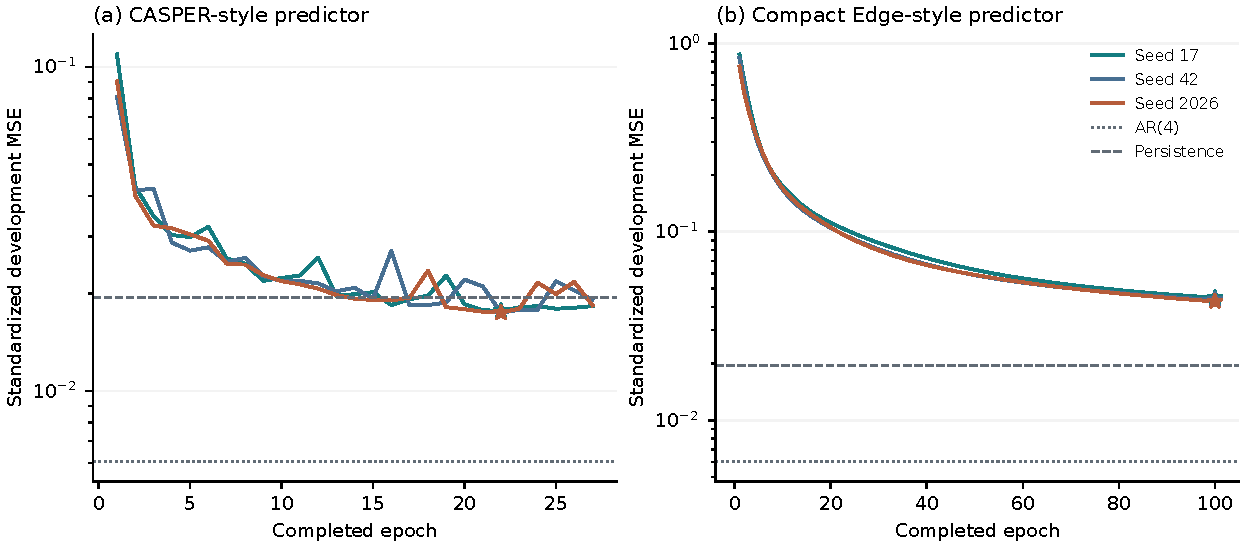
\includegraphics[width=\linewidth]{figures/imu_learning_curves.pdf}
\caption{Normal-development learning curves from the saved training records. Local patience stopping supports greater training adequacy for the CASPER-style architecture; the compact models remain limited by the epoch ceiling. Horizontal control lines refer to the same filtered targets.}\label{fig:imu}
\end{figure}

These results apply to the filtered normal prefix. Median filtering changes the prediction task and introduces dependence, so the autoregressive advantage cannot be assumed to hold for unfiltered attack detection. The patience rule establishes when these runs stopped, not a global optimum, convergence on a representative full dataset or reproduction of the published experiments. This study computes no attack threshold, F1 or recovery score and performs no test-label optimization. Lower normal MSE alone is insufficient evidence of better cyberattack detection.

The run used 764.794 s wall time, 753.252 s CPU, 553.05 MiB sampled peak memory and 2.68 MiB of outputs. Seventeen pre-run synthetic checks and 3,754 fresh-process artifact checks covered checkpoint reloads, score alignment and source identities. The hardware was the same macOS arm64 workstation; process threads and actual budgets are retained in provenance. No neural model was refitted while preparing this manuscript.
